\documentclass[border=12]{standalone}

\usepackage{amsmath}
\usepackage{ifthen}
\usepackage{makecell}
\usepackage{pgfmath}
\usepackage{standalone}
\usepackage{stix}
\usepackage{tikz}
\usepackage{tikz-3dplot}
\usepackage{tkz-euclide}
\usetkzobj{all}
\usetikzlibrary{angles}
\usetikzlibrary{arrows.meta}
\usetikzlibrary{arrows}
\usetikzlibrary{automata}
\usetikzlibrary{calc}
\usetikzlibrary{circuits.logic.IEC}
\usetikzlibrary{circuits.logic.US}
\usetikzlibrary{decorations.footprints}
\usetikzlibrary{decorations.markings}
\usetikzlibrary{decorations.pathmorphing}
\usetikzlibrary{decorations.pathreplacing}
\usetikzlibrary{decorations.shapes}
\usetikzlibrary{decorations.text}
\usetikzlibrary{intersections}
\usetikzlibrary{mindmap}
\usetikzlibrary{patterns}
\usetikzlibrary{positioning}
\usetikzlibrary{quotes}
\usetikzlibrary{shadings}
\usetikzlibrary{shadows}
\usetikzlibrary{shapes.callouts}
\usetikzlibrary{shapes.geometric}
\usetikzlibrary{shapes}

\definecolor{blue1}{RGB}{0,51,255}
\definecolor{green1}{RGB}{0,153,0}
\definecolor{red1}{RGB}{210,35,42}
\definecolor{red2}{RGB}{211,109,85}
\definecolor{yellow1}{RGB}{249,159,52}
\definecolor{yellow2}{RGB}{253,195,130}

%
\definecolor{nagwaBlue}{RGB}{2,107,176}
\definecolor{nagwaFushia}{RGB}{229,29,116}
\definecolor{nagwaGreen}{RGB}{120,181,23}
\definecolor{nagwaYellow}{RGB}{245,170,0}


\begin{document}
	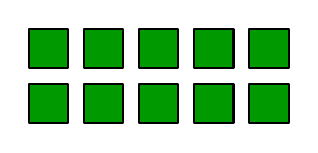
\begin{tikzpicture}
	\begin{scope}[>={Stealth[scale=1.2]},thick, line join=round, font=\fontsize{11.25}{11.25}\selectfont]
	
	\pgfgettransformentries{\mya}{\myb}{\myc}{\myd}{\mys}{\myt}
	\pgfmathsetmacro{\preserve}{1/\mya}
	

\foreach \x in {0,0.7,1.4,2.1,2.8}
\foreach \y in {0,0.7}
{
	\draw [fill=green1] (\x,\y) rectangle +(0.5,0.5);
}

	\end{scope}

	\end{tikzpicture}
\end{document}